% Copy the desired figure environments into report.tex at the suggested locations.
% Paths assume compilation from the repository root. Requires graphicx (already loaded).

% Study 3: Repair Interface
\begin{figure}[tbp]
  \centering
  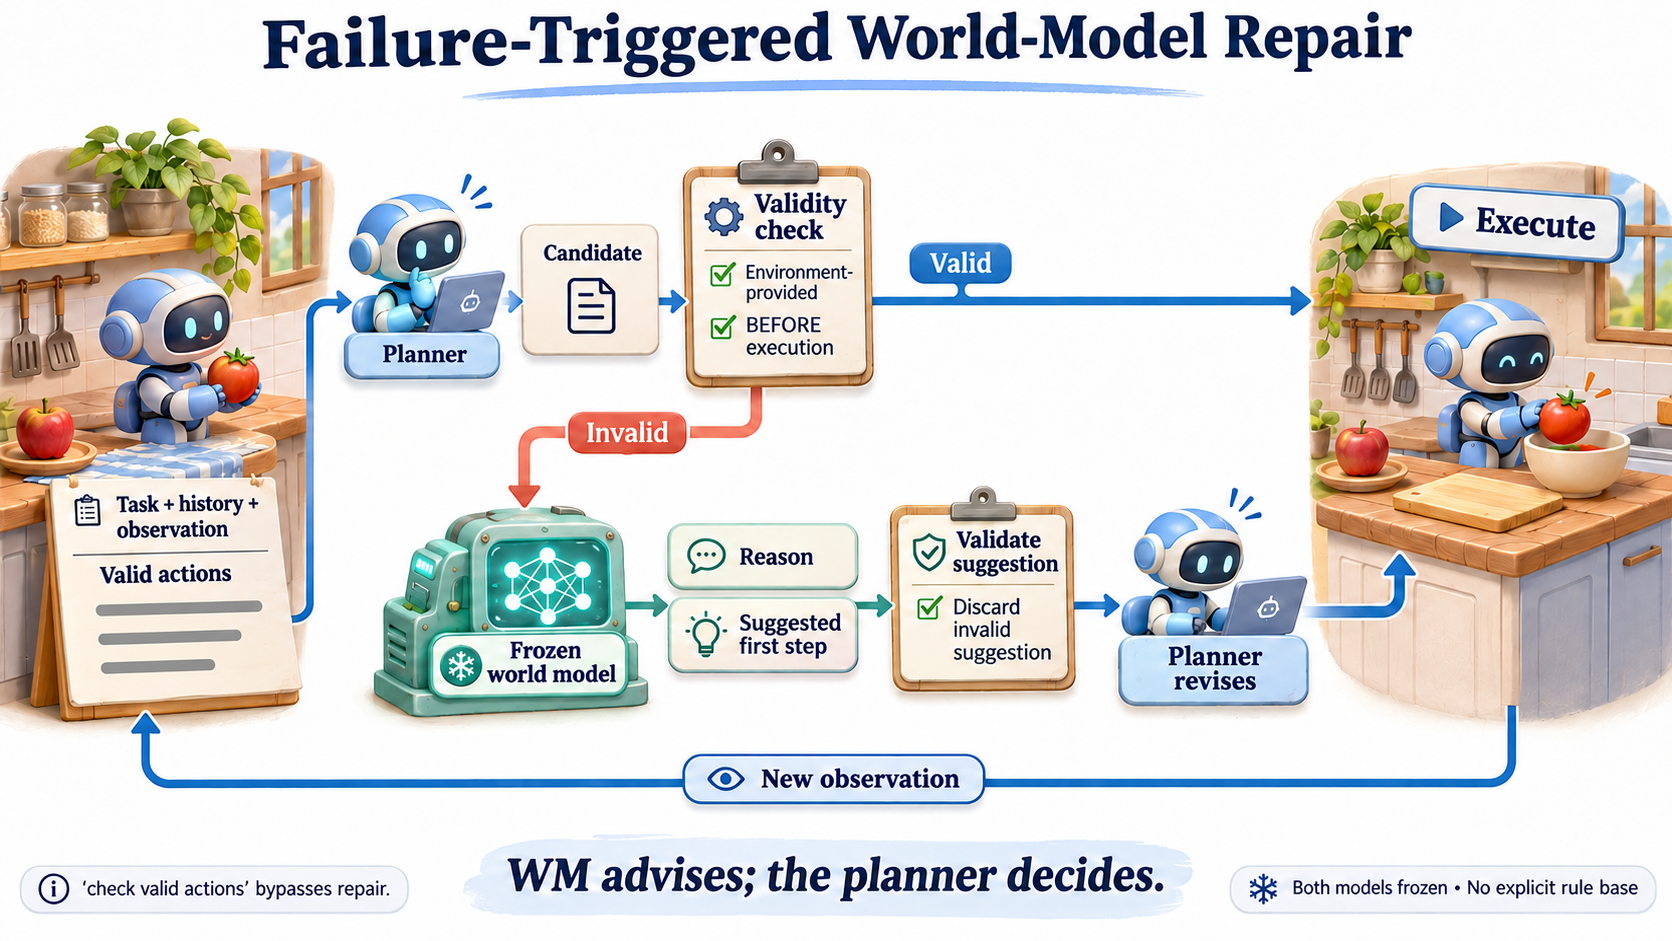
\includegraphics[width=\linewidth]{figures/illustrations/01_method_overview.png}
  \caption{Failure-triggered world-model repair. The environment-provided valid-action list identifies infeasible proposals before execution. The frozen WM supplies a reason and a suggested first step; invalid suggestions are discarded. The planner revises its decision and retains final action selection. The interface command \texttt{check valid actions} bypasses repair and is handled by the interaction protocol. Household scenes are conceptual illustrations.}
  \label{fig:illustrated-wm-repair}
\end{figure}

% Introduction / research progression
\begin{figure}[tbp]
  \centering
  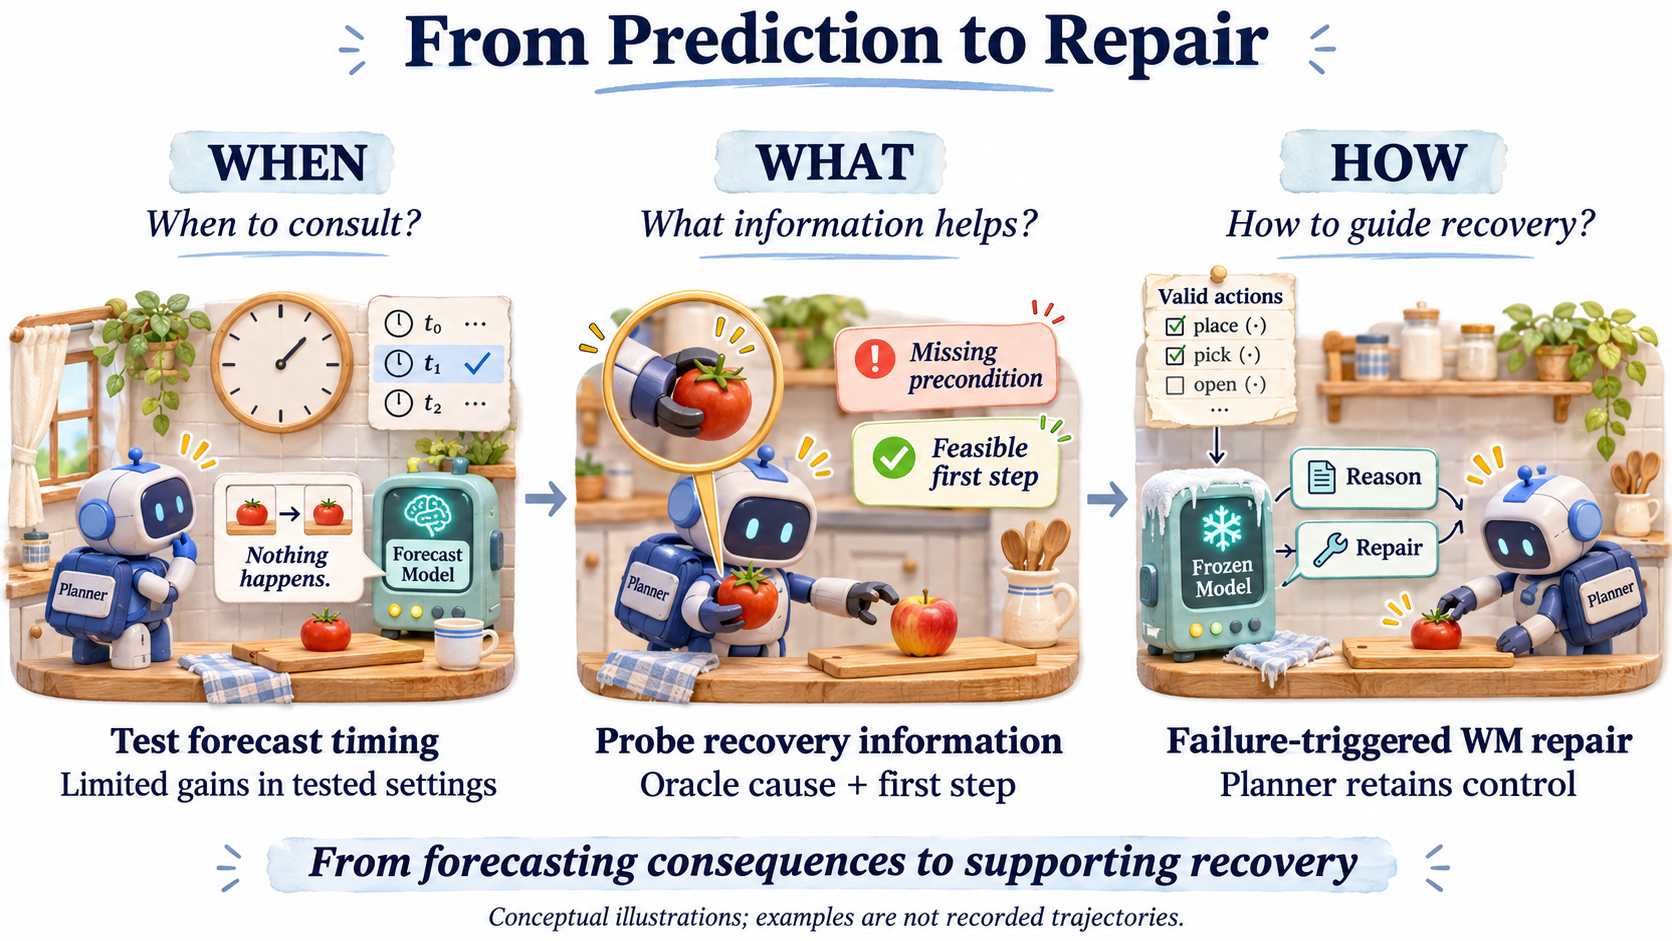
\includegraphics[width=\linewidth]{figures/illustrations/02_when_what_how.png}
  \caption{The WHEN--WHAT--HOW progression: testing forecast timing, identifying recovery information through oracle probes, and delivering repair advice with a frozen WM. Scenes and action-list symbols are conceptual rather than recorded environment states.}
  \label{fig:illustrated-research-progression}
\end{figure}

% Introduction or Study 2: Failure Analysis
\begin{figure}[tbp]
  \centering
  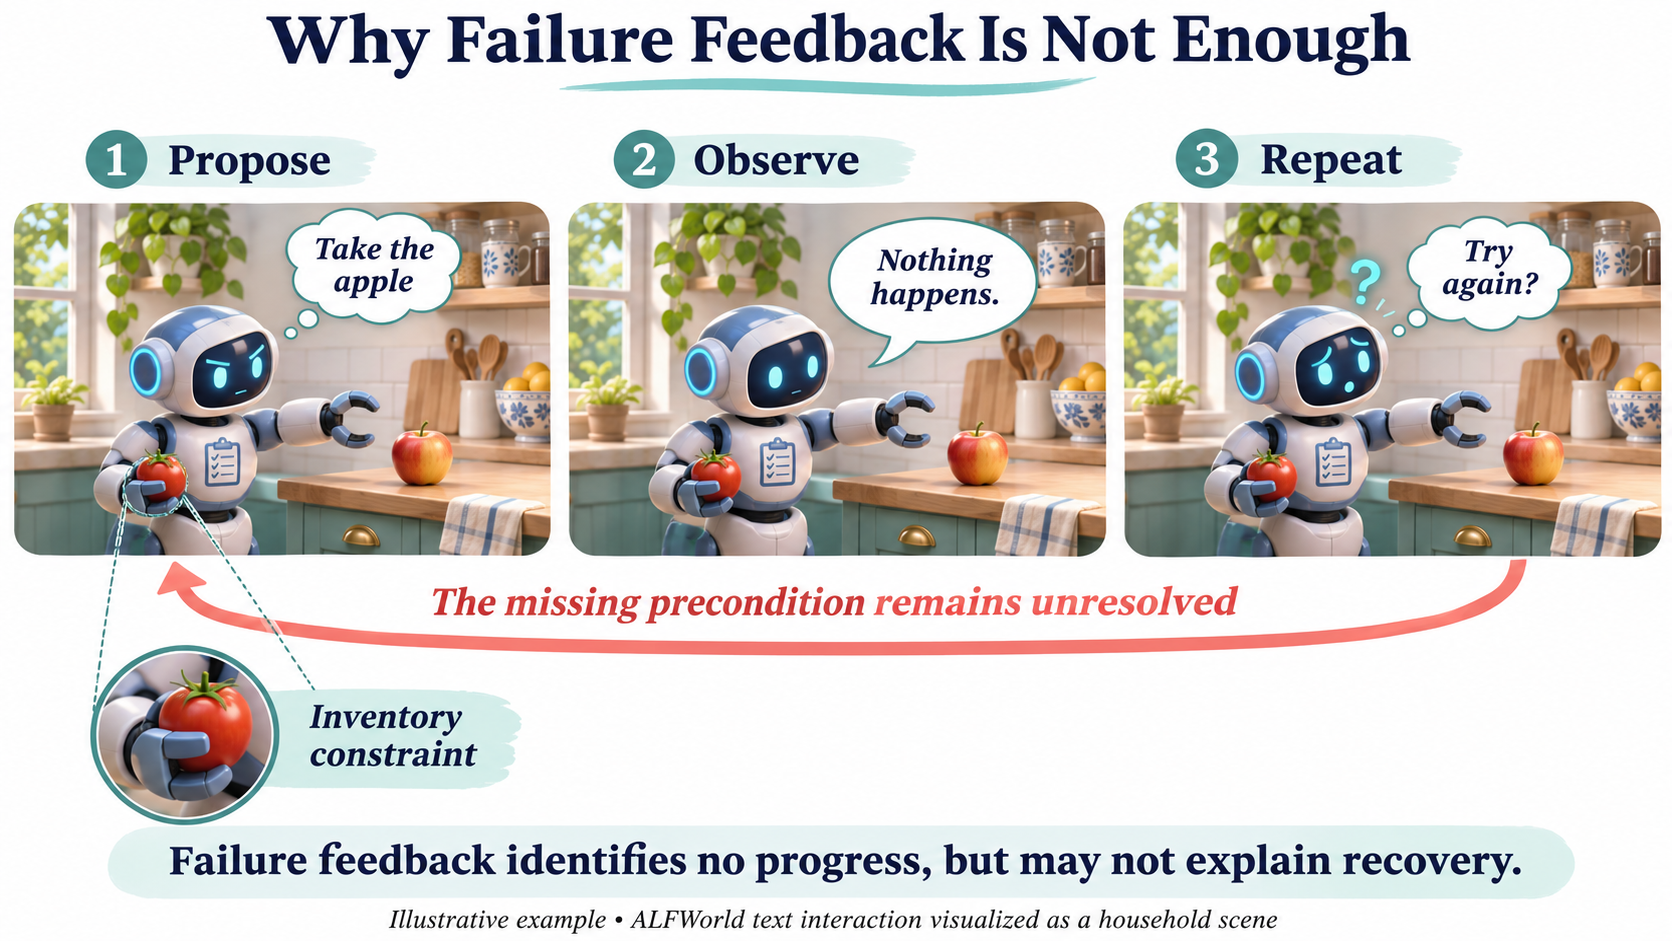
\includegraphics[width=\linewidth]{figures/illustrations/03_failure_loop.png}
  \caption{Illustrative failure loop under an inventory constraint. A planner holding a tomato repeatedly attempts to take an apple; the unchanged observation does not explain the missing precondition. This example illustrates a possible failure mechanism, not an extracted experimental trajectory.}
  \label{fig:illustrated-failure-loop}
\end{figure}

% Study 3: Illustrative interaction
\begin{figure}[tbp]
  \centering
  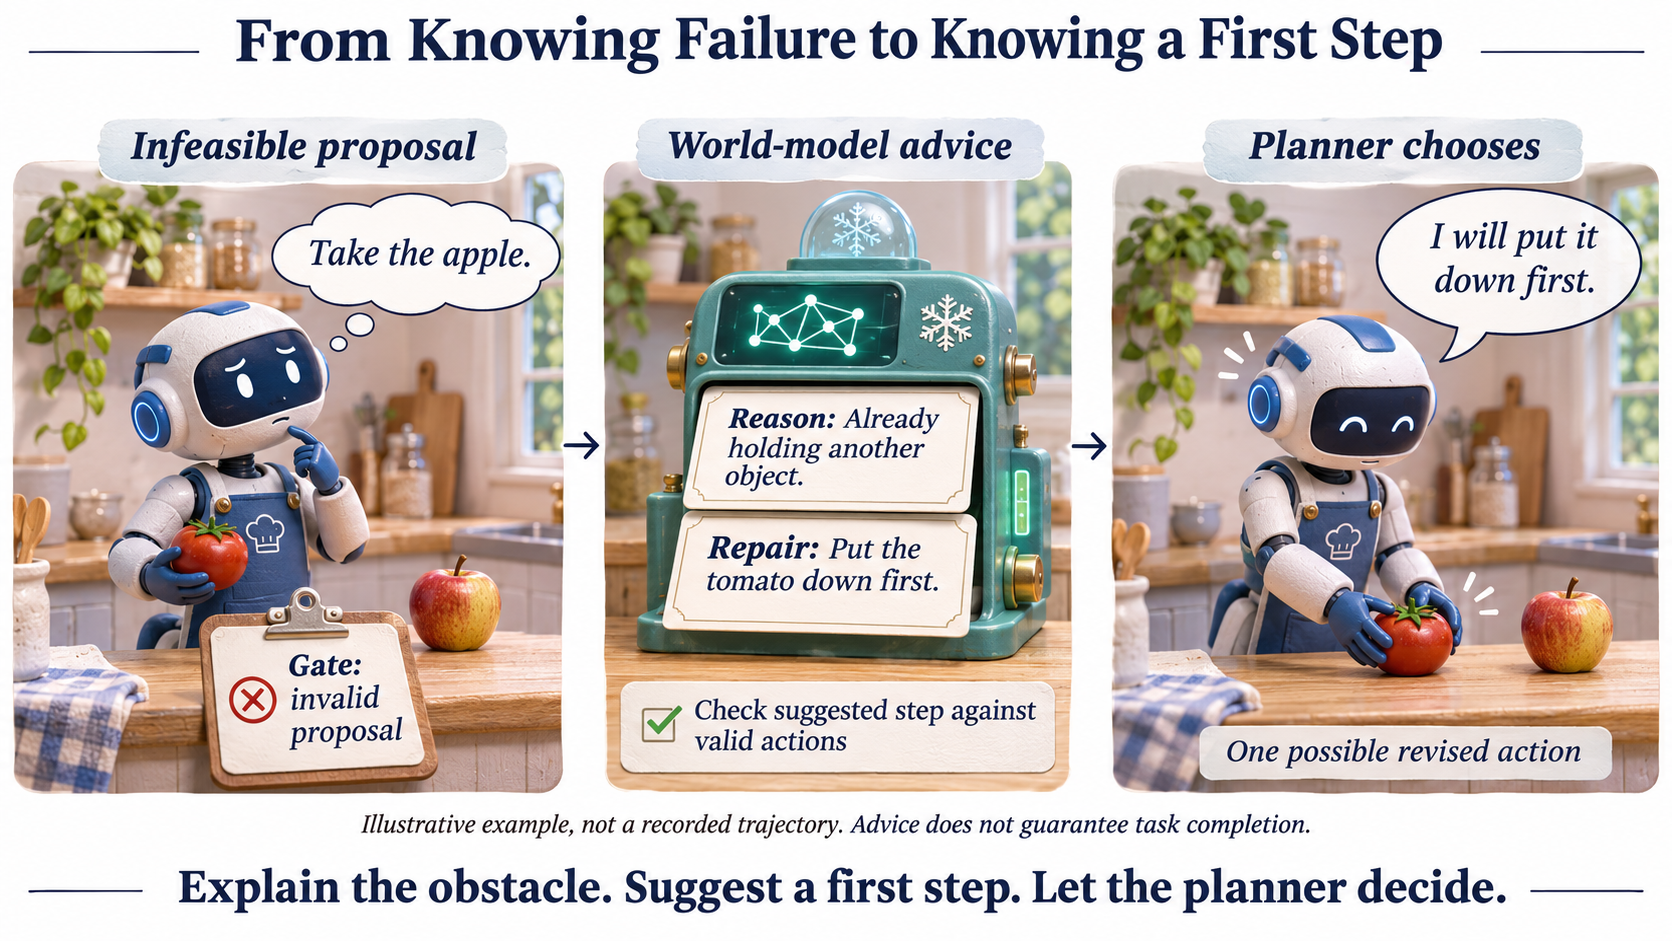
\includegraphics[width=\linewidth]{figures/illustrations/04_repair_example.png}
  \caption{Illustrative repair interaction. The invalid proposal is detected before execution. The WM explains the occupied-inventory constraint and suggests putting down the held object. Following admissibility validation, the planner may choose that first step or another action. Messages are simplified illustrations, not verbatim model outputs or environment commands.}
  \label{fig:illustrated-repair-example}
\end{figure}

% Study 3: Ablation Study
\begin{figure}[tbp]
  \centering
  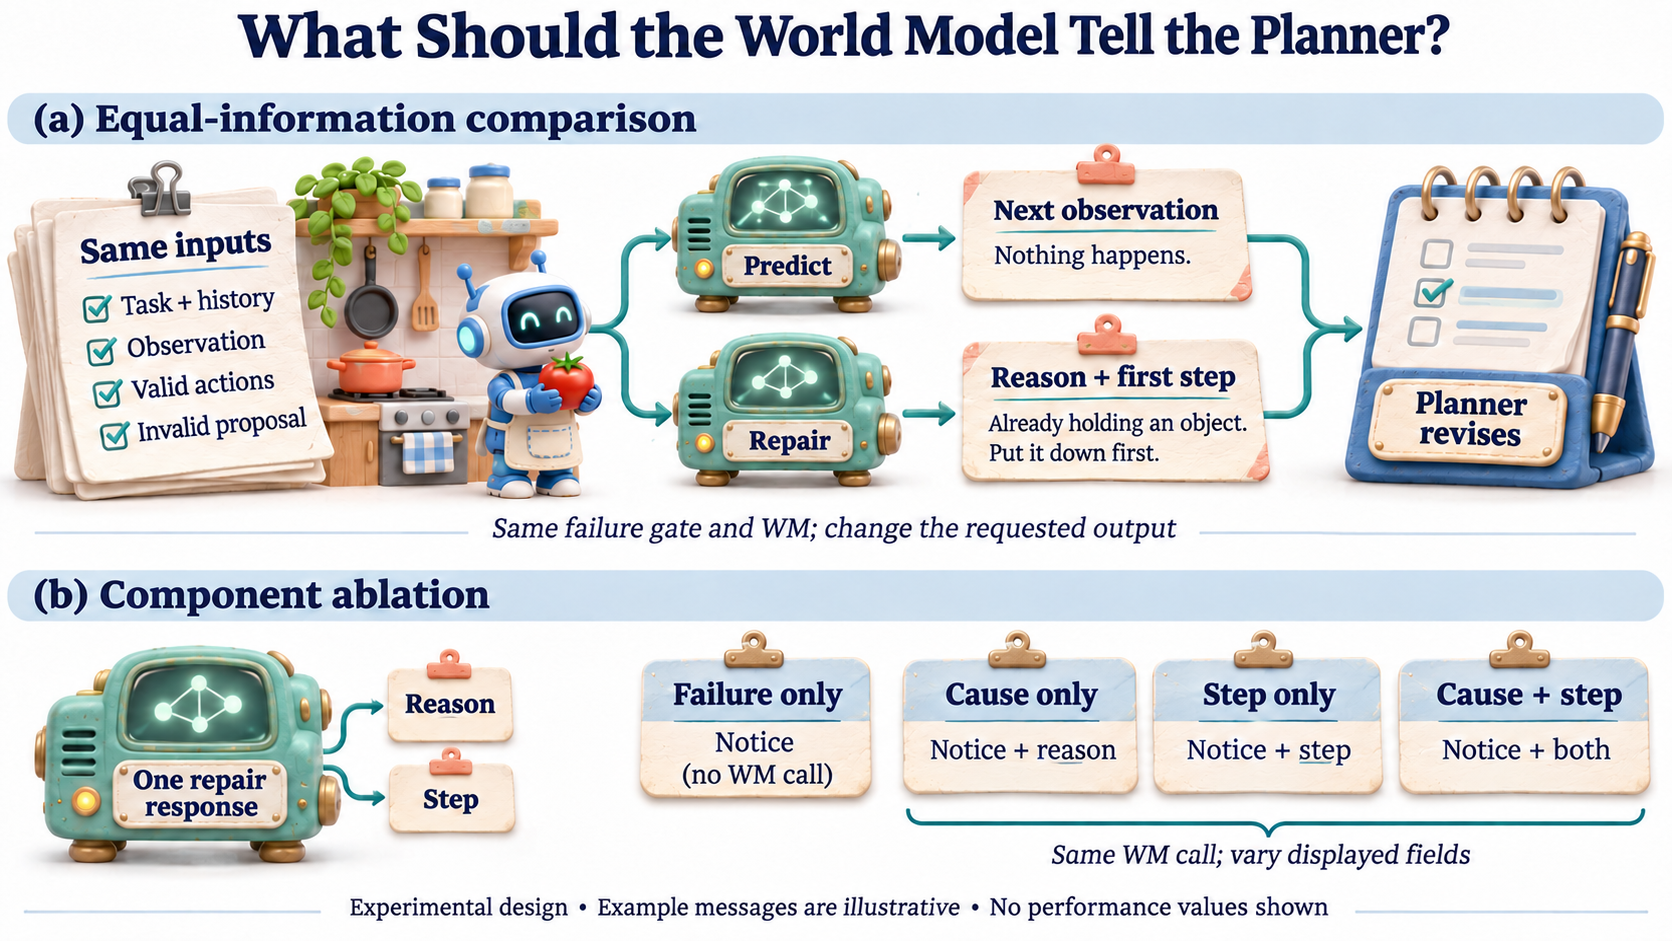
\includegraphics[width=\linewidth]{figures/illustrations/05_interface_ablation.png}
  \caption{Interface ablation design. (a) Equal-information prediction and repair use the same context, WM and failure gate while changing the requested output. (b) Cause-only, step-only and combined advice use the same repair call and vary the fields displayed to the planner. Failure-only is a separate control without a WM call. Example messages are illustrative; the figure does not depict performance measurements.}
  \label{fig:illustrated-interface-ablation}
\end{figure}
